%% =====================================================================
%% BiTeM at the TREC 2026 RAG Track
%%
%% Template and structure: main_knafou_ntcir.pdf (BITEM at NTCIR-19 R2C2),
%% acmart sigconf: Introduction, Related Work, Method (ending with the runs),
%% Results, Discussion and Conclusions; matching the group's VQA notebook paper
%% (repos/trec-vqa/paper/tex/main_bitem_trec_vqa.tex) in its conventions.
%% [nonacm]: TREC proceedings are published by NIST, not ACM.
%%
%% Writing rules (review forwarded 2026-11-09): no revision history, plain terms,
%% round numbers in the text and exact values in the tables, provenance in these
%% comments only. Figures: text at 9 pt or more, drawn at their LaTeX width and
%% included unscaled (figures/make_paper_figures.py checks both, and asserts every
%% plotted value against the numbers printed here).
%% Second review (2026-11-10): title, scope of the citation claim, labelled-only
%% scores are estimates (not bounds), one judge for every list, the depth-matched
%% counterfactual, the passage-window confound, the annotator table.
%% =====================================================================
\documentclass[sigconf,nonacm]{acmart}

\usepackage{booktabs}
\usepackage{multirow}
\usepackage{tikz}
\usetikzlibrary{arrows.meta,fit}

\newcommand{\run}[1]{\mbox{\textbf{#1}}}   %% run tags: bold, never hyphenated
\newcommand{\TBD}[1]{\textcolor{red}{[TBD: #1]}}   %% must be gone before submission
\sloppy
\emergencystretch=2em

%% Numbered citations, as in the NTCIR template this paper follows.
\citestyle{acmnumeric}

\settopmatter{printacmref=false}
\renewcommand\footnotetextcopyrightpermission[1]{}

%% Tighter float spacing, as in the VQA paper.
\setlength{\textfloatsep}{8pt plus 2pt minus 2pt}
\setlength{\floatsep}{8pt plus 2pt minus 2pt}
\setlength{\intextsep}{8pt plus 2pt minus 2pt}
\setlength{\abovecaptionskip}{4pt}
\setlength{\belowcaptionskip}{2pt}

\begin{document}

\title{BiTeM at the TREC 2026 RAG Track: Facet Retrieval, Citation Support and
       the Limits of Self-Built Judges}

\author{Esteban Gaillac, Julien Knafou, Paul Van Rijen, Alexandre Flament, Patrick Ruch}
\affiliation{\institution{HES-SO, Geneva, Switzerland}\country{}}
\affiliation{\institution{SIB Swiss Institute of Bioinformatics, Geneva, Switzerland}\country{}}
\email{esteban.gaillac@hesge.ch}
%% Author block as in the VQA notebook paper of the same group.

\renewcommand{\shortauthors}{Gaillac et al.}

%% ---------------------------------------------------------------- abstract
\begin{abstract}
We took part in both subtasks of the TREC 2026 RAG track with one pipeline run
locally on open-weight models. A model splits each topic into four to six facets,
retrieval runs for every facet and for the whole topic, and the answer is written
facet by facet with every sentence cited. Our primary retrieval run sits at the
median of 114 runs on set precision and above it on set recall, and nine in ten of
the documents it returned came from the facet rankings. \TBD{counterfactual}
The development labels we tuned on were pooled from whole-topic retrieval and
labelled few facet documents, so they could not rank lists built from facet
queries. \TBD{relabelling} All four generation runs are in the bottom half of the
field on the scores released so far, human preference and nugget coverage. The
citation-support scores that the track's guidelines announce, the property we had
optimised, have not been released. Rewriting our development answers for coverage
raised it from 0.36 to 0.49 under our own judges, \TBD{grounded}. Of the judges we
built, the relevance labeller ranked topics as the official judge did but was twice
as lenient, the pairwise judge reversed a third of its verdicts when the answers
were swapped, and the support judge gave full marks to refusals.
\end{abstract}

\keywords{retrieval-augmented generation, query decomposition, rank fusion,
citation support, LLM judges, incomplete relevance judgments}

\maketitle

\section*{Team Name}
BiTeM

\section*{Subtasks}
Retrieval (R) \\
Retrieval-Augmented Generation (RAG)

%% ---------------------------------------------------------------- intro
\section{Introduction}

The TREC 2026 RAG track asks a system to search a corpus and write a cited
answer~\cite{trecrag2026}. The corpus, ClimbMix-400b, is a language-model
pre-training collection reachable only through a search API~\cite{lin2021pyserini}.
Most of the 119 topics are persona-driven scenarios and the rest are plain writing
tasks, from 13 to 206 words long. A single topic asks for priorities, trade-offs,
outcome measures and failure modes at once.
%% 91 of 119 topics carry a first-person pronoun: data/rag/topics/trec_rag_2026_queries.tsv.

One query cannot serve a topic with six parts. Our system has a model write down,
before any retrieval, the facets a complete answer must cover, four to six
sub-topics with their own queries, and every later stage reads that plan.
Everything runs on one A100 with open-weight models and no commercial API, for
reproducibility and cost. With no answer key before the deadline, we also built our
own judges to choose between systems. This paper contributes:
\begin{itemize}\setlength{\itemsep}{1pt}
\item a facet-based retrieval pipeline whose scored rankings are nine-tenths facet
documents, at the field median on set precision and above it on set recall, with
\TBD{counterfactual, one clause};
\item evidence that development labels pooled from whole-topic retrieval cannot
rank lists built from facet queries, including the fusion rule we chose on them,
and a re-scoring of those lists by a single judge;
\item a rewrite of our development answers showing that coverage, as measured in
the scores released so far, credits sentences that their citations do not support,
and a proposal to measure the two together;
\item an account of how four self-built judges compared with the official scores.
\end{itemize}

%% ---------------------------------------------------------------- related
\section{Related Work}

Reciprocal rank fusion sums $1/(k+\mathrm{rank})$ over the lists in which a
document appears~\cite{cormack2009rrf}. Cross-encoders score a query and a passage
jointly and outperform the first-stage ranker they rerank~\cite{nogueira2019passage};
our dense retriever is a bi-encoder of the sentence-embedding
family~\cite{reimers2019sbert, xiao2024cpack}. Our probe-guided system writes an
answer from memory before retrieving, as HyDE~\cite{gao2023hyde} and
query2doc~\cite{wang2023query2doc} do to expand queries; we use the draft to plan
the facets instead.

UMBRELA reproduces a commercial relevance assessor with an open prompt and reports
agreement with human judgments~\cite{upadhyay2024umbrela, thomas2024searcher}, and
the risks of judging with language models are set out in~\cite{faggioli2023perspectives}.
Pairwise judges prefer answers by their position in the prompt~\cite{wang2024fair}
and favour text written by their own model~\cite{panickssery2024selfpref}. The
official retrieval scores rest on UMBRELA labels and on nugget coverage measured
with the AutoNuggetizer framework~\cite{pradeep2024nuggets, pradeep2025greatnugget}.
Earlier editions of the track also scored citations: the 2024 edition judged the
support of each cited sentence by people and by language
models~\cite{thakur2025support}, and the 2025 overview lists attribution
verification among its evaluation layers~\cite{upadhyay2026rag25}. We measured
attribution during development~\cite{gao2023alce}; benchmarks increasingly
separate retrieval quality from answer quality~\cite{yang2024crag}, and entailment
checking against the cited documents tests an answer's claims
directly~\cite{tang2024minicheck}.

Pooling assumes that the union of submitted runs approximates the relevant set, so
a system outside the pool goes unrepresented whatever its
quality~\cite{zobel1998reliable}. Scoring a ranking's condensed list, with the
unjudged documents removed, estimates its score over judged documents
only~\cite{sakai2007alternatives}. This is an estimate, not a bound, and it
flatters lists whose judged documents are the ones the pooled systems also found.
Selecting a system on a metric and then reporting that metric biases the report
upwards~\cite{cawley2010overfitting}; one of our runs does this.

%% ---------------------------------------------------------------- method
\section{Method}

\begin{figure*}[t]
\centering
%% Figure 1: the pipeline, drawn after Figure 1 of main_knafou_ntcir.pdf (grey group panels, white
%% nodes with a bold title and an italic gloss, double borders on the two rules that decide what is
%% submitted, dashed arrows for feedback and the variant). All text is \normalsize, 9 pt in acmart
%% sigconf, the notebook minimum; the picture is drawn at text width (17.8 cm: five 3.1 cm columns
%% and four 0.57 cm gaps) and is not scaled. Glosses repeat figures from the text.
%% Needs tikz with the arrows.meta and fit libraries.
\definecolor{pipeink}{RGB}{52,64,80}
\begin{tikzpicture}[
  font=\normalsize,
  >={Stealth[length=4.5pt,width=4pt]},
  nohyph/.style={execute at begin node={\hyphenpenalty=10000\exhyphenpenalty=10000}},
  panel/.style={rounded corners=4pt, fill=black!4, draw=black!20},
  box/.style={rounded corners=2pt, draw=pipeink, fill=white, line width=0.6pt, align=center,
              minimum height=1.85cm, text width=2.92cm, inner sep=2.5pt, nohyph},
  gate/.style={box, double=white, double distance=1.1pt, line width=0.5pt},
  variant/.style={box, dashed},
  arr/.style={->, draw=pipeink, line width=0.6pt},
  back/.style={->, draw=pipeink, line width=0.6pt, dashed},
  lab/.style={font=\normalsize\itshape, text=black!62, align=left, nohyph},
  ptitle/.style={font=\normalsize\bfseries, anchor=north west},
]
\providecommand{\gl}[1]{\\[1pt]{\itshape #1}}

% ---- panels (drawn first, so everything sits on them)
\draw[panel] (0,0.6) rectangle (14.3,-4.55);
\draw[panel] (3.5,-5.35) rectangle (14.3,-8.85);
\node[ptitle] at (3.62,0.52) {Retrieval};
\node[lab, anchor=north west] at (3.62,0.12) {offline after pooling};
\node[ptitle] at (3.62,-5.43) {Generation};

% ---- retrieval
\node[font=\normalsize\itshape] (topic) at (1.55,1.2) {Topic};
\node[box] (plan) at (1.55,-2.35) {\textbf{Search plan}\gl{4--6 facets and\\ a keyword query}};
\node[box] (pool) at (5.22,-2.35) {\textbf{Pooling}\gl{12 BM25 searches,\\ $\approx$1{,}900 documents}};

\draw[draw=pipeink, fill=white, rounded corners=2pt, line width=0.4pt] (8.89+0.12,-3.45+0.12) ++(-1.55,-0.925) rectangle ++(3.1,1.85);
\draw[draw=pipeink, fill=white, rounded corners=2pt, line width=0.4pt] (8.89+0.06,-3.45+0.06) ++(-1.55,-0.925) rectangle ++(3.1,1.85);
\node[box] (wq) at (8.89,-1.25) {\textbf{Whole topic}\gl{BM25 top 200,\\ reranked by MiniLM}};
\node[box] (fac) at (8.89,-3.45) {\textbf{Facet rankings}\gl{bge top 150 per\\ query; keep 100}};
\node[draw=pipeink, dashed, rounded corners=3pt, line width=0.5pt, inner sep=4pt, fit=(wq)(fac)] (rerank) {};
\node[lab, anchor=south] at (rerank.north) {reranking};

\node[box] (fuse) at (12.56,-1.25) {\textbf{Anchor-first fusion}\gl{whole topic first,\\ facets after}};
\node[gate] (depth) at (12.56,-3.45) {\textbf{Depth rule}\gl{keeps scores $\geq$ the\\ weakest cited one}};
\node[box] (deep) at (16.2,-1.25) {\textbf{Deep rankings}\gl{anchor-first order,\\ not scored}};
\node[box] (scored) at (16.2,-3.45) {\textbf{Scored ranking}\gl{9 in 10 documents\\ from facets}};

\draw[arr] (topic) -- (plan);
\draw[arr] (plan) -- (pool);
\draw[arr] (pool) -- (rerank.west |- pool);
\draw[arr] (wq) -- (fuse);
\draw[arr] (fac) -- (depth);
\draw[draw=pipeink, line width=0.6pt] (10.72,-1.25) -- (10.72,-3.45);
\fill[pipeink] (10.72,-1.25) circle (1.4pt) (10.72,-3.45) circle (1.4pt);
\draw[arr] (fuse) -- (deep);
\draw[arr] (depth) -- (scored);

% ---- probe variant
\node[variant] (probe) at (1.55,-6.75) {\textbf{Probe-guided plan}\gl{from an answer\\ drafted from memory}};
\draw[back] (probe) -- node[lab, right, pos=0.24, text width=1.75cm] {variant: plan from the draft} (plan);

% ---- generation
\node[box] (ctx) at (5.22,-6.75) {\textbf{Context}\gl{whole topic top 10,\\ facets top 6 each}};
\node[box] (syn) at (8.89,-6.75) {\textbf{Synthesis}\gl{one claim per\\ sentence, cited}};
\node[gate] (gates) at (12.56,-6.75) {\textbf{Citation checks}\gl{uncited sentences\\ dropped}};
\node[box] (ans) at (16.2,-6.75) {\textbf{Answer}\gl{bp\_agentic\_v2}};

\draw[arr] (rerank.south) -- ++(0,-0.55) -| node[lab, pos=0.25, above] {top documents} ([xshift=6mm]ctx.north);
\draw[arr] (ctx) -- (syn);
\draw[arr] (syn) -- (gates);
\draw[arr] (gates) -- (ans);
\draw[back] ([xshift=7mm]syn.south) -- ++(0,-0.42) -| node[lab, pos=0.25, below, align=center] {review: one repair round for uncovered facets} ([xshift=-7mm]syn.south);
\draw[back] (gates.north) -- node[lab, left, pos=0.5] {cited documents} (depth.south);
\end{tikzpicture}

\caption{The pipeline. Solid arrows carry data forward; dashed arrows are the
feedback paths and the probe-guided variant; double borders mark the two rules that
decide what is submitted. The scored and the unscored deep rankings come from the
same rankings, ordered and cut differently.}
\label{fig:pipeline}
\end{figure*}

Figure~\ref{fig:pipeline} shows the pipeline. The search plan, the answer and its
repair are written by \texttt{qwen3.5:122b}, an open-weight model served by Ollama.
Retrieval uses bge-large-en-v1.5 embeddings and the ms-marco-MiniLM-L6
cross-encoder.
%% Model names: systems/rag/agentic_v2/pipeline.py (--blueprint-model, --synth-model),
%% tighten.py (embed_model, rerank_model). No citation is attached to qwen3.5: the only
%% Qwen entry in references.bib is the Qwen3 report, which does not cover it.

\subsection{Development data}
We developed on the organisers' 22 development topics, taken from the TREC 2025
track and none of them among the 119 test topics. For these topics the organisers
released relevance labels projected onto ClimbMix by UMBRELA on qwen3.5-9b, with
grades from 0 to 4 and about 1,200 labelled documents per topic. We developed on
their first version (v1); a corrected version (v2) followed on 17 June. Nuggets for
the same topics followed on 12 June, 29 to 90 per topic and 74\% of them vital. The
organisers do not say how the labelled documents were chosen. The labels cover every
document in the top 100 of plain BM25 on the topic text and only 27\% of its ranks
101 to 200, so we take them to come from whole-topic retrieval.
%% data/rag/qrels/*-qwen3.5-9b.qrels (v1), data/rag/qrels_v2/ (v2; README there); 26,341
%% labels / 22 = 1,197. Coverage of plain BM25 (runs/rag/api_climbmix_eval22_fullnarrative.tsv):
%% J@100 = 1.000, J@200 = 0.633, so ranks 101-200 are 26.6% labelled
%% (eval/analysis/team_ideas_2026_11_09.py block 1). Nuggets: data/rag/nuggets/rag25-dev-nuggets.jsonl.
%% trec-rag-skills references/development-data.md describes the files, not the pool.

\subsection{Retrieval}

\subsubsection{Search plan}
One model call per topic returns two to four core entities, four to six facets with
one or two queries each, and a keyword query that compresses the topic into at most
forty words. An earlier system that issued free sub-questions had scored 0.28
nDCG@10~\cite{jarvelin2002cumulated} on the v1 labels against 0.45 for plain
BM25~\cite{robertson2009bm25}. We concluded that sub-questions drift off-topic and
make poor keyword queries, so every generated query must contain the core entities
and be a keyword string. The plan is checked against a schema; without a usable
facet the system falls back to the whole topic.

\subsubsection{Pooling}
The topic text, the keyword query and every facet query go to the API, for 500, 300
and 200 hits. The results are pooled by document id. A topic takes a median of 12
searches, and its pool holds a median of about 1,900 documents (2,500 for the
probe-guided system). Everything after pooling runs offline.
%% eval/analysis/paper_revision_checks.py section 3: median 1,905 (845-2,652) and
%% 2,537 for official119_probe.

\subsubsection{Reranking}
Each topic gets one ranking per facet and one for the whole topic
(Figure~\ref{fig:rerankmap}a--b). For a facet, each query retrieves its 150 nearest
pool documents by bge vector, and the cross-encoder reranks their union against the
facet's queries; the top 100 are kept. For the whole topic, the cross-encoder
reranks the pool's BM25 top 200 against the topic text. The score is an equal mix of
the cross-encoder's sigmoid and the min-max normalised first-stage score. On the v1
labels the mix scored 0.54 nDCG@10 and the cross-encoder alone 0.45.

\begin{figure*}[t]
\centering
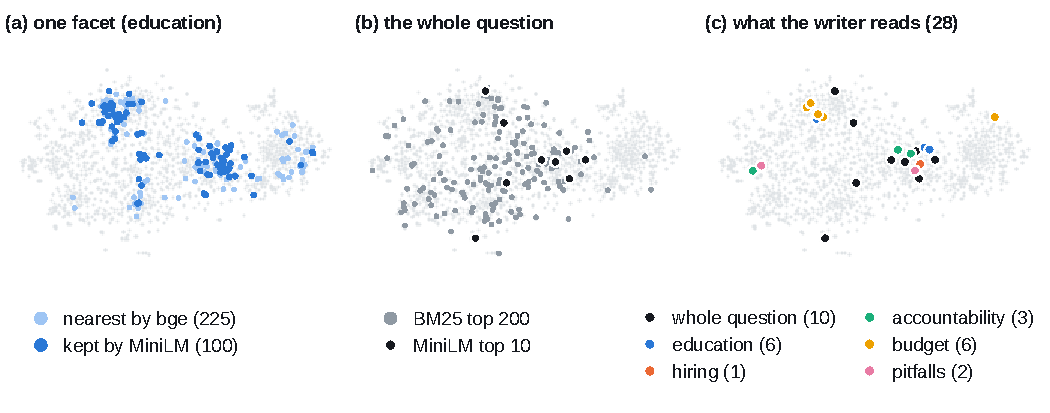
\includegraphics{figures/fig_rerank_map.pdf}
\caption{Reranking and context selection on one topic, rag2026-0 (a hospital
nursing council's three-year diversity plan). Each dot is one of the 1,814
documents pooled for it, placed by its bge vector (t-SNE), so that similar
documents sit close. (a) One facet: the 150 nearest documents to each of its two
queries, 225 in all, and the 100 the cross-encoder keeps. (b) The whole topic: the
pool's BM25 top 200 and the ten the cross-encoder puts first. (c) What the writer
reads: the whole topic's top 10, then each facet's top 6, without repeats.}
\label{fig:rerankmap}
\end{figure*}
%% figures/make_paper_figures.py maps(): candidate sets recomputed as tighten.py
%% builds them and asserted against the cache; counts in figures/paper_figures.json.

\subsubsection{Anchor-first fusion}
The fused ranking copies the whole-topic ranking to its head, appends the facet
rankings combined by reciprocal rank fusion, and fills the rest from the pool in
BM25 order. We chose this order on the v1 labels, where it scored 0.54 nDCG@10
against 0.45 for weighted reciprocal rank fusion of all the lists with the whole
topic at weight two, and 0.53 at weight eight. Fusion that rewards agreement lets a
middling document found by four facet queries outrank the first document of the
whole-topic ranking, and we took that to explain the gap. Not decomposing at all
gives the same top ten on every development topic.
%% 0.449 (w=2), 0.527 (w=8): EXPERIMENTS.md R5, rebuilt from the cached rankings by
%% eval/analysis/fusion_judged_share.py. Whole topic = runs/rag/api_bm25_reranked_full105.tsv.

\subsubsection{Depth rule}
Twelve days before the deadline the organisers asked that each ranking hold the
relevant documents ``and nothing more'' and that its depth be chosen per topic. Our
runs were 1,000 deep with positional scores, and the documents our answers cited sat
around rank 230. We rebuilt the rankings from the reranker scores. A ranking keeps
every document scoring at least as high as the weakest document its answer cites,
which gives a median depth of 100 (18 to 456). A document's score is its best over
all of its topic's rankings, and the kept documents are ordered by it. The facet
rankings score higher than the whole-topic ranking (median 0.58 at rank ten, against
0.32), because each is normalised within its own candidates against a shorter
query. The rule therefore keeps mostly facet documents, and the anchor-first order
survives only in our unscored deep rankings.
%% scripts/build_variable_depth_runs.py (best_ce, policies; rule dated 2026-07-27);
%% cited evidence at median rank 218-247 of the positional runs. Rank-10 medians over
%% the official119 facet_rankings.json files: 0.315 and 0.581.

\subsection{Generation}

\subsubsection{Context}
The writer reads the whole topic's top 10 and each facet's top 6, without repeats:
28 documents for rag2026-0 (Figure~\ref{fig:rerankmap}c). Each document is shown as
its first 700 characters.
%% synthesize.py _passages_block, char_per_doc = 700 for the submitted writer.

\subsubsection{Synthesis and review}
One call writes the answer facet by facet, one claim per sentence and every sentence
cited, in at most 450 words. The prompt asks the model to leave out any facet the
passages cannot support, because ``a shorter fully-grounded answer beats a longer
hedged one''. Both rules served citation support, the property we selected systems
on. A second call lists the facets the answer leaves uncovered, and one repair round
writes sentences for them from up to ten further documents per facet, taken from the
local rankings.
%% systems/rag/agentic_v2/synthesize.py: MAX_WORDS = 450, _SYNTH_SYSTEM, _COVERAGE_SYSTEM.

\subsubsection{Citation checks}
Only documents in the context may be cited. The parser drops ids it cannot resolve
and any sentence left without a valid citation, and the reference list is built from
the citations that survive. Nothing checks during generation that a cited passage
supports its sentence.

\subsection{The probe-guided system}
The probe-guided system changes only the plan. The model first answers the topic
from memory, without retrieval and without hedging, and the plan is derived from
that draft: some facets search for one specific claim of the draft, others for what
it omits. Pooling, reranking, fusion and writing are unchanged.

\subsection{Our judges}
\label{sec:judges-method}
All our judges run prompts and metric code from RAGDoll, the organisers' evaluation
toolkit~\cite{ragdoll}, on local models. The relevance labeller runs the UMBRELA
prompt~\cite{upadhyay2024umbrela} on \texttt{qwen3:32b}~\cite{qwen2025technical} and
reads each document's first 4,000 characters. It produced 46,374 labels on the test
topics, over a pool of our runs, an organiser baseline and a sample of the documents
our depth rule cut. On 981 MS MARCO passages, 250 of them judged relevant by people,
it graded 93\% of the relevant ones 2 or higher, and its specificity was 81\% on hard
negatives and 100\% on random passages. The support judge runs RAGDoll's support
prompt on \texttt{qwen3:32b}. It rates each sentence and cited document as full,
partial or no support (1, 0.5, 0) and reads the document's first 4,000 characters.
The pairwise judge runs RAGDoll's pairwise prompt on \texttt{qwen3.5:122b}, the model
that wrote the answers it compares. The first author read both systems' answers to
each test topic, blind and with sides randomised, and picked one. After the results
we added a nugget judge: RAGDoll's nugget-assignment prompt, parser and metric on
\texttt{qwen3:32b}, against the organisers' development nuggets.
%% Labeller: eval/umbrela_local_label.py; external check:
%% eval/analysis/umbrela_external_calibration/summary.json (93.2%, 80.5%).
%% Support: eval/ragdoll_local_judge.py; pairwise: eval/pairwise_arena_local.py;
%% votes: data/rag/curation/curation.db (annotator: the first author, per the author
%% 2026-11-10); nuggets: eval/nugget_local_judge.py.

\subsection{Runs}
\label{sec:runs}

\subsubsection{Retrieval}
\run{bp\_agentic\_retrieval}, our primary (15,424 rows, median depth 100), and
\run{bp\_probe\_ret}, from the probe-guided system (12,651 rows, median depth 74),
are cut by the depth rule. To enrich the pools, without being scored,
\run{BiTeM\_deep\_v2} and \run{BiTeM\_deep\_probe} give the two systems' anchor-first
rankings before the cut, up to 1,000 documents deep, and \run{BiTeM\_poolenrich}
ranks by our grades the documents we judged relevant that no scored run of ours
returns.
%% Run tags: field 6 of submissions/*/r_output_trec_rag_2026.tsv;
%% submissions/DEEP_POOL_RUNS_README.md.

\subsubsection{Generation}
\run{bp\_agentic\_v2} is our primary and \run{bp\_probe\_guided} the probe-guided
run. \run{bp\_manual\_curated}, our only manual run, takes for each topic the answer
the first author preferred (118 of 119 topics decided). \run{bp\_support\_argmax}
takes for each topic the answer our support judge scored higher, so it is the argmax
of that judge's own measure, as we declared on the submission form.

Two systems appear only on the development topics. The 32B writer is the primary
pipeline with \texttt{qwen3:32b} writing the answer. The agent loop gives the 122B
model tools to search the pool, read documents and take cited notes facet by facet,
and stops when every facet has a note.
%% 67 probe / 51 v2 / 1 skip: data/rag/curation/curation.db, set_kind='manual'.
%% Agent loop: systems/rag/agentic_v2/agent_loop.py (bp_agentic_v3).

%% ---------------------------------------------------------------- results
\section{Results}

The organisers scored retrieval on 82 of the 119 topics and generation on two
batches of 17 and 25. They call the topics narratives and have not released the
judgments behind the scores.

\subsection{Retrieval}
\label{sec:retrieval-results}

\subsubsection{Official scores}
Relevance is an UMBRELA label of 2 or more, assigned by the organisers. Set
precision and set recall are computed at the depth each run chose for each topic,
and nugget gain is the share of a topic's nuggets that at least one returned
document fully supports (Table~\ref{tab:official}). Our primary run sits at the field
median on precision (0.35) and above it on recall (0.17 against 0.10). It is above
the median on recall for 61 of the 82 topics and on precision for 44, at a mean
depth of 131 against a median of 100. Precision does not fall with depth: by thirds
of depth it is 0.37, 0.33 and 0.34.
%% data/rag/official_scores/retrieval_2026-10-29/ (email of 2026-11-02),
%% eval/analysis/official_retrieval_scores.py, FINDINGS_official_retrieval.md.
%% Depth thirds 18-80, 81-154, 155-456; Spearman depth/precision -0.08, p = 0.49.

\begin{table}[t]
\caption{Official retrieval scores: means over the 82 topics judged for documents
and the 25 judged for nuggets. The field columns summarise the 114 evaluated runs of
27 teams; the organisers report no ranks.}
\label{tab:official}
\small
\setlength{\tabcolsep}{4.5pt}
\begin{tabular}{lcccc}
\toprule
 & & & \multicolumn{2}{c}{field} \\
\cmidrule(lr){4-5}
 & primary & probe-guided & median & max \\
\midrule
set precision & 0.3456 & 0.3042 & 0.3499 & 0.7297 \\
set recall & 0.1659 & 0.1108 & 0.1002 & 0.5475 \\
mean depth & 131.3 & 100.3 & 100 & 4{,}541.6 \\
gain, NIST nuggets & 0.8987 & 0.8743 & 0.8965 & 0.9837 \\
gain, automatic nuggets & 0.6521 & 0.5192 & 0.6268 & 0.9229 \\
\bottomrule
\end{tabular}
\end{table}

The primary beats the probe-guided run on precision for 54 topics against 28
(exact sign test, $p = 0.005$) and on recall for 59 against 23 ($p < 0.001$),
although the probe-guided run returns fewer documents. Its facets send retrieval
after claims the model drafted from memory, including invented ones. For rag2026-113
the draft described a television episode, ``Neural Drift'', that does not exist,
and the plan searched for its title, cast and plot. On the automatic nuggets the
primary beats the field median on 15 of 25 topics and the probe-guided run on 18 of
the 23 where they differ ($p = 0.011$). The NIST nuggets barely separate runs, since
the field median already reaches full gain on 12 of 25 topics. Our deep rankings add
128,990 document--topic pairs to the pools, 121,457 of which nobody had labelled.
%% data/rag/cache/agentic_v2/official119_probe/rag2026-113/{draft,blueprint}.json.
%% 128,990 / 121,457: (deep_v2 U deep_probe) minus (both scored runs U poolenrich),
%% then minus data/rag/cache/umbrela_labels.jsonl; SUBMISSION_FORM_ANSWERS.md:94.

\subsubsection{What the scored rankings contain}
Of the 15,424 documents in our primary run, 13,958 are absent from their topic's
whole-topic ranking, 88\% of each list on average. In rag2026-0, 187 of 197 take
their score from a facet ranking (Figure~\ref{fig:scoredmap}). The share is 92\% in
the probe-guided run. Facet documents also make up 78\% of the documents our
answers cite. Our labeller calls 68\% of the primary's whole-topic documents relevant
and 64\% of its facet-only ones. In the probe-guided run the figures are 70\% and
54\%, which fits its lower official precision.
%% eval/analysis/team_ideas_2026_11_09.py block 5 (labels cover every submitted
%% document); probe: 871 whole-topic and 11,780 facet-only documents. Cited documents
%% outside the whole-topic list: official119 answer.json citations, mean 0.783.

\begin{figure}[t]
\centering
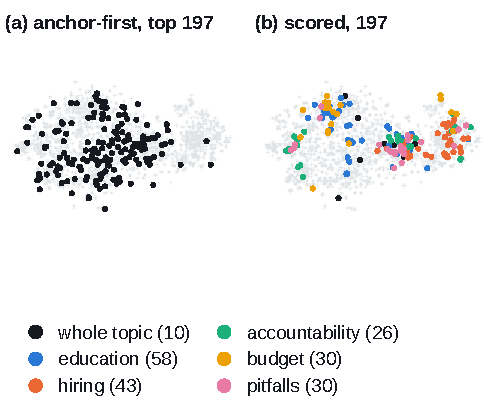
\includegraphics{figures/fig_scored_map.pdf}
\caption{What was scored for rag2026-0, on the map of Figure~\ref{fig:rerankmap}.
(a) The first 197 documents of the anchor-first ranking, all from the whole topic.
(b) The 197 documents of the scored run, coloured by the ranking that gave each its
score.}
\label{fig:scoredmap}
\end{figure}

\subsubsection{Facet documents against the whole topic at the same depth}
\TBD{depth-matched counterfactual: our labeller, 82 topics, scored run against the
anchor-first ranking cut at the same depth}

\subsubsection{Headroom}
From the official per-topic precision $P$ and recall $R$ at our depth $k$, a topic
has $Pk/R$ relevant documents in the judged pool: a median of 206, while we returned
a median of 98 documents, 30 of them relevant. A perfect ranking at our depth would
have reached a median recall of 0.48. On the development topics, which have a mean
of 693 relevant documents each, our pool contains 39\% of them. Reranking keeps 200
documents for the whole topic and 100 per facet, which drops 44\% of the relevant
documents in the pool, and the final top 1,000 holds 30\%.
%% eval/analysis/paper_revision_checks.py section 4; team_ideas_2026_11_09.py block 4.

\subsubsection{Mainstream and niche topics}
Are some topics too mainstream for the model? We measured how much the corpus holds
on a topic by its number of relevant documents in the official pool, $Pk/R$ (25 to
1,503). The probe-guided run's recall falls further behind the primary's on topics
with few relevant documents, but most of that is arithmetic, since the same shortfall
is a larger share of a small set. In relevant documents found, the gap is unrelated
to the measure (Spearman $-0.04$). The ratio of the two recalls shows a trend (0.29,
$p = 0.009$) that does not survive correction for the ten tests we ran. Neither do
two other trends: on topics with many relevant documents our precision and our
answers' coverage fall further below the field median (Spearman $-0.28$ and $-0.42$,
$p = 0.011$ and $0.035$).
%% eval/analysis/team_ideas_2026_11_09.py block 3; hits and recall-ratio checks of
%% 2026-11-10 (review): rho -0.036 (p 0.75) and +0.290 (p 0.0086), n = 81; the raw
%% recall difference gave +0.416. Coverage: batch-2 automatic nuggets, 25 topics.

\subsection{What the development labels can rank}
\label{sec:dev-labels}
Table~\ref{tab:fusion} repeats the development comparisons behind our design with
two additions: the share of each top ten that carries a label, and the score over
labelled documents only, which estimates what the label gaps hide but is no bound.
The labels cover 98\% of the anchor-first top ten and 74\% of the fused top ten at
weight two. Over labelled documents only, reciprocal rank fusion scores 0.53 and
anchor-first 0.50 on the v2 labels, within noise. The cross-encoder alone matches the
score mix, and the free sub-questions fall 2 points behind BM25 instead of 14. The
comparisons between fully labelled lists do not move: reranking the whole topic
beats plain BM25, and MiniLM beats the larger bge reranker.
\TBD{our labeller on every top ten: P@10 per row and paired differences}
%% eval/analysis/fusion_judged_share.py (rows rebuilt and re-scored; the RRF rows
%% reproduce EXPERIMENTS.md R5); v2 paired anchor-first minus RRF x2: +0.074 (SE 0.026)
%% over all documents, -0.029 (SE 0.020) over labelled documents only.

\begin{table}[t]
\caption{Development topics (22), nDCG@10 under the organisers' projected labels,
v1 and v2, counting unlabelled documents as non-relevant. Labelled: share of the top
ten with a label. Labelled only: nDCG@10 (v2) over labelled documents, an estimate
that favours lists resembling the labels' pool. RRF rows are rebuilt from the cached
rankings; the last row uses the 568M bge reranker.}
\label{tab:fusion}
\small
\setlength{\tabcolsep}{2.8pt}
\begin{tabular}{lcccc}
\toprule
 & \multicolumn{2}{c}{nDCG@10} & & labelled \\
\cmidrule(lr){2-3}
ranking & v1 & v2 & labelled & only \\
\midrule
anchor-first (ours) & 0.5352 & 0.4985 & 98\% & 0.5048 \\
whole topic only & 0.5352 & 0.4985 & 98\% & 0.5048 \\
RRF, whole topic $\times$2 & 0.4493 & 0.4245 & 74\% & 0.5333 \\
RRF, whole topic $\times$8 & 0.5273 & 0.4944 & 96\% & 0.5148 \\
cross-encoder alone & 0.4501 & 0.4021 & 81\% & 0.5003 \\
\midrule
naive sub-questions & 0.2794 & 0.2810 & 70\% & 0.4002 \\
plain BM25 & 0.4483 & 0.4238 & 100\% & 0.4238 \\
\midrule
anchor-first, bge reranker & 0.4832 & 0.4456 & 100\% & 0.4456 \\
\bottomrule
\end{tabular}
\end{table}

Below rank ten the picture is the same (Figure~\ref{fig:ranks}). Anchor-first and
the whole-topic ranking are the same list down to rank 200 on 21 of the 22 topics,
and the facet documents show only below it, where recall at 1,000 is 0.30 against
0.25. The order of our scored runs has 32\% of its top ten labelled. Its precision at
ten is 0.30 with unlabelled documents counted as misses and 0.93 over labelled
documents only, so the development labels cannot place it. Applied to the
development topics, the depth rule keeps a median of 168 documents, 90\% of them from
facet rankings, and 28\% of the kept documents carry a label.
%% eval/analysis/team_ideas_2026_11_09.py block 1 and its JSON; identical top-200
%% lists on 21/22 topics (the 22nd overlaps 99.8%).

\begin{figure}[t]
\centering
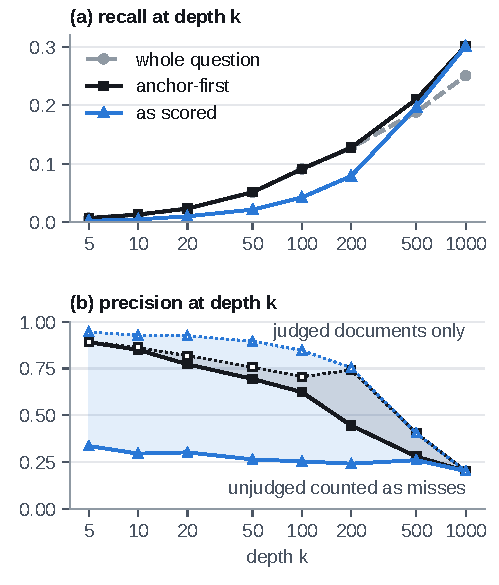
\includegraphics{figures/fig_ranks.pdf}
\caption{Development topics at depth $k$, organisers' v2 labels, relevant meaning
grade 2 or more. (a) Recall. (b) Precision with unlabelled documents counted as
misses (solid) and over labelled documents only (dotted). ``As scored'' is the order
of our scored runs before the depth cut.}
\label{fig:ranks}
\end{figure}

Replaying the reranking on the development topics reproduces the cached rankings
exactly, and Figure~\ref{fig:stages} scores each ranking before and after the
cross-encoder. On the whole topic, where nearly every document has a label, the
cross-encoder raises precision at ten from 0.70 to 0.85. On the facet rankings,
where fewer than a third of the top ten have one, neither the cross-encoder nor
reranking against the whole topic can be compared with the bge order on these
labels.
%% eval/analysis/team_ideas_2026_11_09.py block 6 (replay: whole-topic top ten
%% identical on 22/22 topics, every position of the 200, 100% of each facet's 100).

\begin{figure}[t]
\centering
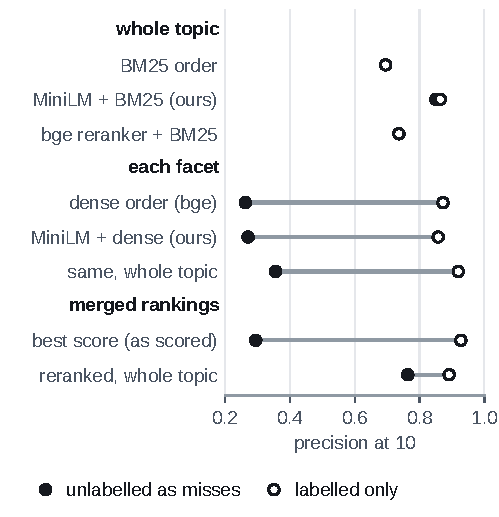
\includegraphics{figures/fig_stages.pdf}
\caption{Each ranking before and after reranking, development topics: precision at
ten with unlabelled documents counted as misses (filled) and over labelled documents
only (open). ``Ours'' is the submitted recipe.}
\label{fig:stages}
\end{figure}

%% ---------------------------------------------------------------- generation
\subsection{Generation}
\label{sec:gen-results}

\subsubsection{Official scores}
NIST assessors compared answers side by side on 17 topics in batch~1 and 25 in
batch~2, for each team's two priority runs, and the organisers fitted a
Bradley--Terry rating to their choices. All four runs were also scored on coverage,
the share of a topic's nuggets that the answer fully supports. The nuggets are
rubric criteria written by assessors in batch~1, and in batch~2 nuggets written by
assessors and nuggets generated automatically, all assigned to answers by GPT-6.1
Sol~\cite{pradeep2024nuggets}. The track's guidelines also announce weighted citation
precision and recall, organiser-run, from 29 July~\cite{trecrag2026guidelines}. The
scores released so far do not include them, and the organisers' description of the
released scores never mentions citations.
%% data/rag/official_scores/generation_2026-11-03/README_nour_rag_gen.md. Guidelines:
%% TREC-RAG/trec-rag-skills, references/rag-task.md, section "Evaluation"; the support
%% paragraph first appears in commit f281e88 (2026-07-29), absent from 246d0348,
%% 18942820, 499c15f4, 6fe3f2a3 and f3428f37. Official figures here:
%% eval/analysis/official_generation_scores.py, FINDINGS_official_generation.md.

\begin{table*}[t]
\caption{Official generation scores. Human preference is a Bradley--Terry rating with
its 95\% interval, assessed only for each team's two priority runs. Coverage is the
share of a topic's nuggets the answer fully supports; ``vital'' counts only the
essential ones. Field columns summarise all evaluated runs.}
\label{tab:officialgen}
\small
\begin{tabular}{lcccccc}
\toprule
 & primary & probe-guided & annotator picks & support picks & \multicolumn{2}{c}{field} \\
\cmidrule(lr){6-7}
 & bp\_agentic\_v2 & bp\_probe\_guided & bp\_manual\_curated & bp\_support\_argmax & median & max \\
\midrule
human preference, batch 1 & 834.8 [781, 889] & 847.0 [792, 902] & --- & --- & 1048.7 & 1258.2 \\
human preference, batch 2 & 924.1 [884, 964] & 850.7 [805, 896] & --- & --- & 1024.8 & 1261.7 \\
\midrule
rubric, batch 1, vital & 0.6069 & 0.6520 & \textbf{0.7157} & 0.6098 & 0.7157 & 0.8922 \\
rubric, batch 1, all & 0.5750 & 0.5662 & \textbf{0.6334} & 0.5298 & 0.7325 & 0.9115 \\
NIST nuggets, vital & \textbf{0.4774} & 0.3934 & 0.4348 & 0.4065 & 0.4879 & 0.7286 \\
NIST nuggets, all & \textbf{0.4882} & 0.4012 & 0.4613 & 0.4113 & 0.5556 & 0.7804 \\
automatic nuggets, vital & 0.1321 & 0.1217 & \textbf{0.1487} & 0.1274 & 0.1547 & 0.6656 \\
automatic nuggets, all & 0.1040 & 0.0960 & \textbf{0.1184} & 0.0992 & 0.1280 & 0.5840 \\
\bottomrule
\end{tabular}
\end{table*}

All four runs are in the bottom half of the field on every released measure
(Table~\ref{tab:officialgen}), except the manual run, which reaches the median on the
batch-1 vital criteria. Assessors preferred the other system's answer in 530 of our
765 decided comparisons. No measure separates the primary and the probe-guided runs
significantly. The probe-guided run is ahead on the batch-1 ratings and vital
criteria and behind on the NIST nuggets (13 topics to 6, $p = 0.17$).
Our answers use about a third of the 1,024-word limit (medians of 286 and 366 words),
and the organisers' baselines run 564 to 680 words. Within our runs, longer answers
cover more automatic nuggets (Spearman 0.33, $p = 0.019$). The probe-guided run
writes longer answers without scoring higher, so length is a candidate cause only.
The coverage judge is not fully repeatable: of 125 answers scored twice, six received
different scores. Our own support judge had put the four runs between 0.82 and 0.84,
except \run{bp\_support\_argmax} at 0.87, which leads by construction.
%% Our support figures (weighted precision, all judged citations): v2 0.8198,
%% probe 0.8370, manual 0.8158, argmax 0.8694; all 6,657 citations resolve.

\subsubsection{Rewritten answers}
\label{sec:revised}
We wrote for citation support, and the scores released so far measure coverage and
preference. After the results we tested the obvious change on the 22 development
topics, with a design fixed in writing beforehand. The documents the submitted
pipeline retrieved stay; only the writer changes, and our nugget judge scores
coverage. Each variant adds one change to the one before (Table~\ref{tab:rerun}).
The first runs the submitted writer again, to measure noise. The second raises the
cap to 950 words and doubles the sentence target. The third replaces the two rules
written for support with a prompt to cover every facet with specific facts. The
fourth shows each document as its best-matching 1,000 characters instead of its first
700. The last raises coverage from 0.36 to 0.49, 6.8 standard errors of the paired
difference, while running the submitted writer again moves it by 0.01.

\begin{table*}[t]
\caption{Development answers (22 topics) on the organisers' development nuggets,
coverage of all nuggets by our nugget judge. $\ddagger$: written after the official
results from the same documents, never submitted; each adds to the row above.
$\Delta$: paired difference from the submitted answers, in standard errors.
Supported: share of sentences with at least one fully supporting citation, by our
support judge reading the cited document's first 4,000 characters or the passage the
writer was shown. Grounded: coverage counting only those sentences.}
\label{tab:rerun}
\small
\begin{tabular}{lccccccccc}
\toprule
 & & & & & \multicolumn{2}{c}{judge reads first 4,000} & \multicolumn{2}{c}{judge reads passage shown} \\
\cmidrule(lr){6-7}\cmidrule(lr){8-9}
writer & coverage & $\Delta$ (SE) & vital & words & supported & grounded & supported & grounded \\
\midrule
submitted & 0.356 & --- & 0.393 & 268 & 83\% & 0.305 & \TBD{} & \TBD{} \\
run again$^\ddagger$ & 0.367 & $+0.011$ (1.4) & 0.402 & 274 & --- & --- & --- & --- \\
950-word cap$^\ddagger$ & 0.379 & $+0.023$ (1.3) & 0.411 & 396 & --- & --- & --- & --- \\
coverage prompt$^\ddagger$ & 0.439 & $+0.083$ (4.8) & 0.465 & 647 & \TBD{} & \TBD{} & \TBD{} & \TBD{} \\
best passages$^\ddagger$ & 0.488 & $+0.132$ (6.8) & 0.510 & 636 & 65\% & 0.382 & \TBD{} & \TBD{} \\
weights, reviews$^\ddagger$ & 0.490 & $+0.134$ (8.3) & 0.523 & 762 & 68\% & 0.383 & \TBD{} & \TBD{} \\
\midrule
32B writer & 0.380 & $+0.023$ (1.3) & 0.410 & 253 & --- & --- & --- & --- \\
agent loop & 0.384 & $+0.028$ (1.4) & 0.419 & 217 & --- & --- & --- & --- \\
probe-guided & 0.323 & $-0.034$ (1.6) & 0.353 & 376 & --- & --- & --- & --- \\
\bottomrule
\end{tabular}
\end{table*}
%% eval/analysis/PREREG_post_results_rerun.md (design, addenda A and B, results);
%% scripts/run_synth_arms.py; eval/nugget_local_judge.py; eval/analysis/
%% nugget_dev22_{existing,arms,multipass,grounded,review}.json; supported/grounded:
%% eval/analysis/grounded_coverage_dev22.py and review_checks_2026_11_10.py support-shown.

\TBD{grounding paragraph: both judges; window confound; coverage-prompt row}

\begin{figure}[t]
\centering
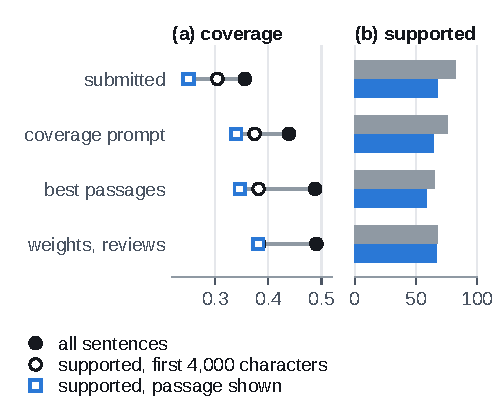
\includegraphics{figures/fig_grounded.pdf}
\caption{\TBD{caption after the shown-passage results}}
\label{fig:grounded}
\end{figure}

Weighting the facets and reviewing the answer several times, each time asking what
is still uncovered, changed coverage by $+0.002$ against the best-passages writer (9
topics up, 11 down) for 126 more words. The test is weak, because the model gave the
top weight to 103 of the 111 facets and the reviews found something to repair on 9
of the 22 topics. The single review of the submitted writer repaired 23\% of
development topics and 33\% of test topics, and 95\% of the probe-guided system's
test topics, whose draft-planned facets the context covers worst. The nugget judge
puts the 32B writer and the agent loop slightly above the submitted writer, within
noise, and the probe-guided system below it, also within noise. We rewrote the
answers to the 42 test topics judged for generation in the same way, so that they can
be scored if the organisers release their nuggets.
%% Multipass: addendum A of PREREG_post_results_rerun.md; repair counts:
%% team_ideas_2026_11_09.py block 2; official rewrite: scripts/run_evidence_official119.sh,
%% runs/rag/bp_v2_evidence_official119_judged42.jsonl.

%% ---------------------------------------------------------------- judges
\subsection{Our judges against the official scores}
\label{sec:judges}

\subsubsection{The relevance labeller}
Our labels cover every document we submitted, so we recomputed set precision from
them at the submitted depths. Their per-topic precision follows the official one
(Spearman 0.78 for the primary run, 0.80 for the probe-guided run), and they order our
two runs correctly. They are lenient. Of the primary's 10,767 documents, our labeller
calls 7,191 relevant and the official judge 3,661, so mean precision is 0.64 against
0.35. A linear fit gives official $\approx 0.72 \times \text{ours} - 0.11$. Our
labels serve relative comparisons, and every absolute precision or recall we derived
from them was about twice too high. Both judges are automatic, so this compares two
runs of the same prompt, and says nothing about agreement with people.
%% eval/analysis/official_retrieval_scores.py; FINDINGS_official_retrieval.md.

\subsubsection{The pairwise judge}
On the 22 development pairs that the pairwise judge saw in both orders, it reversed
its verdict on 7 when the answers were swapped. In a three-candidate comparison on
the 119 test topics, it declared a tie on 26 topics, which the order of the
command-line arguments then decided. Its favourite system was the agent loop, which
returned eight empty answers. The judge also compared answers written by its own
model, a setting in which language models favour their own text. We submitted no run
built from its choices, so the official scores cannot check it.
%% Reversals: logs/calib/seed_model_verdicts_20260727_114350.log and curation.db
%% (set_name 'dev22_v2_vs_probe'): probe 12, primary 3, 7 ties that are reversals.
%% Official 119 audit: EXPERIMENTS.md G7; runs/rag/bp_agentic_v3_official119.
%% support_judgments.jsonl (eight empty answers).

\subsubsection{The support judge}
\label{sec:refusal}
Topic rag2026-113 asks for an invented television episode. The probe-guided answer
begins ``There is no evidence in the provided passages confirming the existence of
\ldots{}'' and scores full support, 1.00, and the primary's answer, which delivers a
titled premise, scores 0.78. Any refusal is supported by the passage it cites. The
judge also gave full support to four sentences consisting of a single full stop.
Picking per test topic the best-supported of three candidates overrides the pairwise
judge's choice on 87 topics. On 44 of those it picks the probe-guided answer, from
the system whose answers hold 4.5 times as many readable defects over the 119 topics
(50 sentences against 11): bare punctuation, leaked facet labels and sentence
fragments. Against the official scores, the support judge's picks do no better than
chance (Table~\ref{tab:annotator}), and \run{bp\_support\_argmax} is last or second
to last of our runs on every measure.
%% runs/rag/best_of_support_aware_official119.jsonl (arena_winner vs selected_from);
%% eval/detect_text_defects.py on bp_agentic_v2_official119{,_probe}.jsonl.

\subsubsection{The annotator}
The first author preferred the probe-guided answers 67 to 51 ($p = 0.17$), with sides
balanced (left 65, right 53), and agreed with the pairwise judge on 13 of the 15
topics where both decided. Against our support judge the votes picked the
better-supported answer on 43 of 112 topics ($p = 0.018$), and we withdrew the manual
run from priority before submission. Table~\ref{tab:annotator} sets the votes and the
support judge's picks against each official measure, on the topics where the two
candidates scored differently. The votes did best on the batch-1 rubric, 12 of 14
($p = 0.013$), and were close to chance on the NIST nuggets, 11 of 19. The manual run
trails the primary on the NIST nuggets (0.46 against 0.49). One annotator, and an
author, on 14 to 24 topics per measure is thin evidence; a second annotator on the
same pairs is the cheapest way to firm it up.
%% data/rag/curation/curation.db; 43/112 against eval/analysis/rejudge_final/
%% summary.json; table: official_generation_scores.py section 4.

\begin{table}[t]
\caption{Picking per test topic between the primary and the probe-guided answer: how
often the first author's blind votes and our support judge picked the answer the
official measure scored higher, on topics where the two scored differently, with an
exact sign test. Coverage measures count all nuggets.}
\label{tab:annotator}
\small
\setlength{\tabcolsep}{3pt}
\begin{tabular}{lcccc}
\toprule
 & \multicolumn{2}{c}{annotator} & \multicolumn{2}{c}{support judge} \\
\cmidrule(lr){2-3}\cmidrule(lr){4-5}
official measure & right & $p$ & right & $p$ \\
\midrule
rubric, batch 1 & 12 of 14 & 0.013 & 5 of 14 & 0.42 \\
NIST nuggets, batch 2 & 11 of 19 & 0.65 & 8 of 19 & 0.65 \\
automatic nuggets, batch 2 & 14 of 19 & 0.064 & 9 of 19 & 1.00 \\
side by side, batch 1 & 7 of 14 & 1.00 & 7 of 14 & 1.00 \\
side by side, batch 2 & 16 of 24 & 0.15 & 11 of 24 & 0.84 \\
\bottomrule
\end{tabular}
\end{table}

\subsection{Process failures}
\label{sec:process}
An audit four days before the deadline found 75 defective sentences in runs that had
passed every validator: leaked facet labels, sentences consisting of a full stop, and
answers cut mid-word. A judging run pointed at the wrong cache left 624 of the
probe-guided run's 1,895 citations unjudged without raising an error; on the 40
topics free of such citations the two systems are level (0.84 and 0.83). An internal
comparison that put the probe-guided answers ahead 7 to 3 had used 10 of the 22
development topics, because a sample argument defaulted to 10. Thirty-four sentences
in runs declared automatic had been written by a person during repairs, and we
regenerated them and disclosed two remaining per-topic human judgements. The
citation parser attaches a citation placed after a full stop to the next sentence, so
the first claim loses its citation and is deleted; we did not keep the raw outputs to
count how often. We also missed the corrected development labels of 17 June, which
move our development nDCG@10 from 0.54 to 0.50, and the development nuggets of
12 June, which would have let us measure coverage before submitting.
%% Defects: SUBMISSION_FORM_ANSWERS.md:131; clean-40 from the pre_mergedroot.bak
%% judgments; 7-3: logs/calib/seed_model_verdicts_20260727_114350.log; parser:
%% systems/rag/generate.py _parse_answer, paper_revision_checks.py section 5.

%% ---------------------------------------------------------------- discussion
\section{Discussion and Conclusions}
\label{sec:discussion}

The track asks for answers in which every sentence cites its evidence, and its
guidelines announce citation scores. The scores released so far judge only what an
answer says. We built for citation support and selected systems on it, and the
released measures do not score it. \TBD{grounding sentence for the discussion}
Neither measure is enough alone, since citation support is maximised by refusing to
answer and coverage by asserting. They combine cheaply, because RAGDoll contains both
a support judge and a nugget assigner: a nugget could count only when a sentence that
states it cites a document that supports it.

Our development labels were pooled from whole-topic retrieval, and at each design
decision we preferred the option that resembled that pool: keyword queries over
sub-questions, the score mix over the cross-encoder alone, anchor-first fusion over
reciprocal rank fusion. Over labelled documents only, all three gaps shrink to
within noise or close to it. Anchor-first fusion was the choice those labels could not
fault, and we have not shown that it was the better one. \TBD{one sentence from the
relabelling and the counterfactual} Labels projected from another pool rank the
systems that resemble the pool; the share of each top ten that carries a label is a
cheap check of that.

We trusted the support judge over the annotator, and the official coverage scores
agree more often with the annotator, most clearly on the batch-1 rubric. Comparing
self-built judges with one another shows where they disagree and not which is right.
We chose the 122B writer over the 32B one, and the fixed pipeline over the agent loop,
in pairwise battles under a judge that reverses a third of its verdicts when the
answers are swapped. On the development nuggets neither choice is better than its
alternative.

\subsection{Requests to the organisers}
\begin{itemize}\setlength{\itemsep}{1pt}
\item Release the citation-support scores the guidelines announce, and report
coverage over supported sentences next to plain coverage.
\item Release the relevance judgments and nugget assignments behind the released
scores, so that deep rankings and post-hoc runs can be scored.
\item Name the judge models, so that teams can calibrate their own judges.
\item Publish how each subtask will be scored before submission; the depth rule
came twelve days before the deadline, and the measure for the ranked list with the
scores.
\item Document how development labels were pooled, or label lists from outside the
pool.
\item Note that gain on the NIST nuggets is near its ceiling: the median run reaches
full gain on 12 of 25 topics.
\end{itemize}

\subsection{What we would do differently}
In retrieval we would pool deeper, since 61\% of the development topics' relevant
documents never enter our pool. We would tune on the measure that is scored, set
precision and recall at the chosen depth, and label the gaps in the development
labels with one judge before comparing lists built from different queries. We would
give every document one comparable score before choosing the depth, and calibrate
our labeller against official labels first. In generation we would write for
coverage and measure grounding beside it, and give the facets weights the model has
to ration. In evaluation we would build the development judge for what will be
scored, as the development nuggets allowed from June, and check every judge against a
person before trusting it.

\subsection{Conclusions}
Facet retrieval produced most of what was scored and reached the field median on
precision and above it on recall. \TBD{conclusion sentence on the counterfactual}
Our generation runs, built for citation support, sit in the bottom half on the
measures released so far, and our rewrite shows that coverage alone also credits
sentences their citations do not back. Our self-built judges were least reliable
exactly where we leaned on them most, in choosing between our own systems. Code,
our runs and the analysis and figure scripts are at
\url{https://github.com/ecsltae/trec2026-rag}.

\bibliographystyle{ACM-Reference-Format}
\bibliography{references}

\end{document}
